\documentclass{article}
\usepackage{amsmath,amssymb,amsthm,mathtools}
\usepackage{tikz-cd}

\begin{document}

\title{Issue XXIV: Category Theory}
\author{Максим Сохацький $^1$}
\date{ $^1$ Національний технічний університет України \\
       \small Київський політехнічний інститут імені Ігоря Сікорського \\
       \today }
\maketitle

\begin{abstract}

Formal definition of Category.

{\bf Keywords}: Category Theory \\
\end{abstract}

\ifincludeTOC
  \tableofcontents
\fi

\section{Category Theory}

Category Theory provides a rigorous framework for abstracting and unifying mathematical structures.
Developed in the 1940s by Samuel Eilenberg and Saunders Mac Lane to address coherence problems in
algebraic topology, it generalizes relationships between mathematical objects across diverse fields
like algebra, geometry, and computer science. Category Theory captures objects and their
morphisms—functions preserving structure—as a universal systems theory,
akin to a universal algebra of functions, emphasizing composition and transformation.
Interpreted as a foundational language, a tool for structural analysis,
or a bridge to computer-aided formalization, it solves problems of abstraction and generalization.
Categories serve as a stepping stone to topos theory, which enriches logical and geometric insights,
and higher cohesive topos theory, extending to infinity-categories for advanced applications.


\newpage
\subsection{Category}

First of all very simple category theory up to pullbacks is provided. We give here
all definitions only to keep the context valid.

A \textbf{category} $\mathcal{C}$ consists of:
\begin{itemize}
  \item A class of \textbf{objects}, $\mathrm{Ob}(\mathcal{C})$,
  \item A class of \textbf{morphisms}, $\mathrm{Hom}_{\mathcal{C}}(X,Y)$, for each pair $X,Y \in \mathrm{Ob}(\mathcal{C})$,
  \item Composition maps $\circ: \mathrm{Hom}(Y,Z) \times \mathrm{Hom}(X,Y) \to \mathrm{Hom}(X,Z)$,
  \item Identity morphisms $\mathrm{id}_X \in \mathrm{Hom}(X,X)$ for each $X$,
\end{itemize}
satisfying associativity and identity laws.

\begin{definition} (Category Signature). The signature of category is
a $\sum_{A:U}A \rightarrow A \rightarrow U$ where $U$ could be any universe.
The $\mathrm{pr}_1$ projection is called $\mathrm{Ob}$ and $\mathrm{pr}_2$ projection is
called $\mathrm{Hom}(a,b)$, where $a,b:\mathrm{Ob}$.
\begin{lstlisting}
cat: U = (A: U) * (A -> A -> U)
\end{lstlisting}
\end{definition}

\begin{definition} (Precategory). More formal, precategory $\mathrm{C}$ consists of the following.
(i) A type $\mathrm{Ob}_C$, whose elements are called objects;
(ii) for each $a,b: \mathrm{Ob}_C$, a set $\mathrm{Hom}_C(a,b)$, whose elements are called arrows or morphisms.
(iii) For each $a: \mathrm{Ob}_C$, a morphism $1_a : \mathrm{Hom}_C(a,a)$, called the identity morphism.
(iv) For each $a,b,c: \mathrm{Ob}_C$, a function
     $\mathrm{Hom}_C(b,c) \rightarrow \mathrm{Hom}_C(a,b) \rightarrow \mathrm{Hom}_C(a,c)$
     called composition, and denoted $g \circ f$.
(v) For each $a,b: \mathrm{Ob}_C$ and $f: \mathrm{Hom}_C(a,b)$, $f = 1_b \circ f$ and $f = f \circ 1_a$.
(vi) For each $a,b,c,d: A$ and $f: \mathrm{Hom}_C(a,b)$, $g: \mathrm{Hom}_C(b,c)$, $h: \mathrm{Hom}_C(c,d)$,
     $h \circ (g \circ f ) = (h \circ g) \circ f$.
\begin{lstlisting}
def cat : U₁
 := Σ (ob: U) (hom: ob -> ob -> U), unit

def isPrecategory (C: cat) : U := Σ
    (id:      Π (x: C.ob), C.hom x x)
    (∘:       Π (x y z: C.ob),
                C.hom x y -> C.hom y z -> C.hom x z)
    (homSet:  Π (x y: C.ob), isSet (C.hom x y))
    (∘-left:  Π (x y: C.ob) (f: C.hom x y),
              = (C.hom x y) (∘ x x y (id x) f) f)
    (∘-right: Π (x y: C.ob) (f: C.hom x y),
              = (C.hom x y) (∘ x y y f (id y)) f)
    (∘-assoc: Π (x y z w: C.ob) (f: C.hom x y)
                (g: C.hom y z) (h: C.hom z w),
              = (C.hom x w) (∘ x z w (∘ x y z f g) h)
                            (∘ x y w f (∘ y z w g h))), 1
def precategory: U₁ := Σ (C: cat) (P: isPrecategory C), unit

\end{lstlisting}

\newpage
Univalent Categories:

\begin{lstlisting}

def isoCat (P: precategory) (A B: P.C.ob) : U := Σ
    (f: P.C.hom A B)
    (g: P.C.hom B A)
    (retract: Path (P.C.hom A A) (P.P.∘ A B A f g) (P.P.id A))
    (section: Path (P.C.hom B B) (P.P.∘ B A B g f) (P.P.id B)), 1

def isCategory (P: precategory): U
 := Σ (A: P.C.ob), isContr (Π (B: P.C.ob), isoCat P A B)

def category: U₁
 := Σ (P: precategory), isCategory P
\end{lstlisting}
\end{definition}

\newpage
\subsection{Pullback}

\begin{definition} (Categorical Pullback).
The pullback of the cospan $A \mapright{f} C \mapleft{g} B$ is a object $A \times_{C} B$ with
morphisms $pb_1 : \times_C \rightarrow A $, $pb_2 : \times_C \rightarrow B$, such that
diagram commutes:
\begin{center}
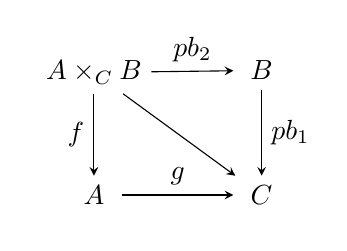
\begin{tikzpicture}
  \matrix (m) [matrix of math nodes,row sep=3em,column sep=3em,minimum width=2em]
  {
     A \times_{C} B & B \\
     A & C\\};
  \path[-stealth]
    (m-1-1) edge node [above] {$pb_2$} (m-1-2)
            edge node [above] {$$} (m-2-2)
    (m-1-1) edge node [left]  {$f$} (m-2-1)
    (m-1-2) edge node [right] {$pb_1$} (m-2-2)
    (m-2-1) edge node [above] {$g$} (m-2-2);
\end{tikzpicture}
\end{center}
Pullback $(\times_C,pb_1,pb_2)$ must be universal, means for any $(D,q_1,q_2)$
for which diagram also commutes there must exists a unique $u: D \rightarrow \times_C$,
such that $pb_1 \circ u = q_1$ and $pb_2 \circ q_2$.
\begin{lstlisting}
def homTo  (P: precategory) (X: P.C.ob): U
 := Σ (Y: P.C.ob), P.C.hom Y X

def cospan (P: precategory): U
 := Σ (X: P.C.ob) (_: homTo P X), homTo P X

def hasCospanCone (P: precategory) (D: cospan P) (w: P.C.ob) : U
 := Σ (f: P.C.hom w D.2.1.1) (g: P.C.hom w D.2.2.1),
    = (P.C.hom w D.1) (P.P.∘ w D.2.1.1 D.1 f D.2.1.2)
                      (P.P.∘ w D.2.2.1 D.1 g D.2.2.2)
def cospanCone (P: precategory) (D: cospan P): U
 := Σ (w: P.C.ob), hasCospanCone P D w

def isCospanConeHom (P: precategory) (D: cospan P)
    (E1 E2: cospanCone P D) (h: P.C.hom E1.1 E2.1) : U
 := Σ (_ : = (P.C.hom E1.1 D.2.1.1)
             (P.P.∘ E1.1 E2.1 D.2.1.1 h E2.2.1) E1.2.1),
           = (P.C.hom E1.1 D.2.2.1)
             (P.P.∘ E1.1 E2.1 D.2.2.1 h E2.2.2.1) E1.2.2.1

def cospanConeHom (P: precategory) (D: cospan P) (E1 E2: cospanCone P D) : U
 := Σ (h: P.C.hom E1.1 E2.1), isCospanConeHom P D E1 E2 h

def isPullback (P: precategory) (D: cospan P) (E: cospanCone P D) : U
 := Σ (h: cospanCone P D), isContr (cospanConeHom P D h E)

def hasPullback (P: precategory) (D: cospan P) : U
 := Σ (E: cospanCone P D), isPullback P D E
\end{lstlisting}
\end{definition}

\newpage
\subsection{Functor}

A \textbf{functor} $F: \mathcal{C} \to \mathcal{D}$ assigns to each:
\begin{itemize}
  \item Object $X \in \mathcal{C}$ an object $F(X) \in \mathcal{D}$,
  \item Morphism $f: X \to Y$ a morphism $F(f): F(X) \to F(Y)$,
\end{itemize}
such that $F(\mathrm{id}_X) = \mathrm{id}_{F(X)}$ and $F(g \circ f) = F(g) \circ F(f)$.


\begin{definition} (Category Functor).
Let $A$ and $B$ be precategories.
A functor $F : A \rightarrow B$ consists of: (i) A function $F_{Ob}: Ob_hA \rightarrow Ob_B$;
(ii) for each $a,b:Ob_A$, a function $F_{Hom}:Hom_A(a,b)\rightarrow Hom_B(F_{Ob}(a),F_{Ob}(b))$;
(iii) for each $a:Ob_A$, $F_{Ob}(1_a) = 1_{F_{Ob}}(a)$;
(iv) for $a,b,c:Ob_A$ and $f: Hom_A(a,b)$ and $g: Hom_A(b,c)$, $F(g\circ f) = F_{Hom}(g)\circ F_{Hom}(f)$.
\begin{lstlisting}
def catfunctor (A B: precategory): U
 := Σ (ob: A.C.ob -> B.C.ob)
      (mor:   Π (x y: A.C.ob),
                A.C.hom x y -> B.C.hom (ob x) (ob y))
      (id:    Π (x: A.C.ob),
              = (B.C.hom (ob x) (ob x))
                (mor x x (A.P.id x)) (B.P.id (ob x)))
      (fcomp: Π (x y z: A.C.ob) (f: A.C.hom x y) (g: A.C.hom y z),
              = (B.C.hom (ob x) (ob z))
                (mor x z (A.P.∘ x y z f g))
                (B.P.∘ (ob x) (ob y) (ob z) (mor x y f) (mor y z g))), 1

\end{lstlisting}
\end{definition}

\newpage
\subsection{Terminals}
\begin{definition} (Terminal Object). Is such object $\mathrm{Ob}_C$,
that
$$
    \prod_{x,y:\mathrm{Ob}_C} \mathrm{isContr} (\mathrm{Hom}_C(y,x)).
$$
\begin{lstlisting}
def isInitial (P: precategory) (bot: P.C.ob): U
 := Π (x: P.C.ob), isContr (P.C.hom bot x)

def isTerminal (P: precategory) (top: P.C.ob): U
 := Π (x: P.C.ob), isContr (P.C.hom x top)

def initial (P: precategory): U
 := Σ (bot: P.C.ob), isInitial P bot

def terminal (P: precategory): U
 := Σ (top: P.C.ob), isTerminal P top
\end{lstlisting}
\end{definition}

\newpage
\subsection{Natural Transformation}
A \textbf{natural transformation} $\eta: F \Rightarrow G$ between functors $F, G: \mathcal{C} \to \mathcal{D}$ consists of morphisms $\eta_X: F(X) \to G(X)$ such that for every $f: X \to Y$ in $\mathcal{C}$,
\[
\begin{tikzcd}
F(X) \arrow[r, "\eta_X"] \arrow[d, "F(f)"'] & G(X) \arrow[d, "G(f)"] \\
F(Y) \arrow[r, "\eta_Y"'] & G(Y)
\end{tikzcd}
\]
commutes.
\begin{lstlisting}
def isNaturalTransformation
    (C D: precategory)
    (F G: catfunctor C D)
    (eta: Π (x: C.C.ob), D.C.hom (F.ob x) (G.ob x)) : U
 := Π (x y: C.C.ob) (h: C.C.hom x y),
    = (D.C.hom (F.ob x) (G.ob y))
      (D.P.∘ (F.ob x) (F.ob y) (G.ob y) (F.mor x y h) (eta y))
      (D.P.∘ (F.ob x) (G.ob x) (G.ob y) (eta x) (G.mor x y h))

def nattrans (C D: precategory) (F G: catfunctor C D): U
 := Σ (η: Π (x: C.C.ob), D.C.hom (F.ob x) (G.ob x))
      (commute: isNaturalTransformation C D F G η), unit

def natiso (C D: precategory) (F G: catfunctor C D) : U
 := Σ (left: nattrans C D F G)
      (right: nattrans C D G F), 1
\end{lstlisting}

\newpage
\subsection{Adjunction}
An \textbf{adjunction} between categories $\mathcal{C}$ and $\mathcal{D}$ consists of functors
\[
F: \mathcal{C} \leftrightarrows \mathcal{D} : G
\]
and natural transformations (unit $\eta$ and counit $\varepsilon$)
\[
\eta: \mathrm{Id}_{\mathcal{C}} \Rightarrow G \circ F, \quad \varepsilon: F \circ G \Rightarrow \mathrm{Id}_{\mathcal{D}}
\]
satisfying the triangle identities.
\begin{lstlisting}
ntransL (C D: precategory) (F G: catfunctor C D)
        (f: ntrans C D F G) (B: precategory) (H: catfunctor B C)
      : ntrans B D (compFunctor B C D H F) (compFunctor B C D H G)
      = (eta, p) where
        F': catfunctor B D = compFunctor B C D H F
        G': catfunctor B D = compFunctor B C D H G
        eta (x: carrier B): hom D (F'.1 x) (G'.1 x) = f.1 (H.1 x)
        p (x y: carrier B) (h: hom B x y): Path (hom D (F'.1 x) (G'.1 y))
            (compose D (F'.1 x) (F'.1 y) (G'.1 y) (F'.2.1 x y h) (eta y))
            (compose D (F'.1 x) (G'.1 x) (G'.1 y) (eta x) (G'.2.1 x y h))
          = f.2 (H.1 x) (H.1 y) (H.2.1 x y h)

ntransR (C D: precategory) (F G: catfunctor C D)
    (f: ntrans C D F G) (E: precategory) (H: catfunctor D E)
  : ntrans C E (compFunctor C D E F H) (compFunctor C D E G H)
  = (eta, p) where
    F': catfunctor C E = compFunctor C D E F H
    G': catfunctor C E = compFunctor C D E G H
    eta (x: carrier C): hom E (F'.1 x) (G'.1 x)
      = H.2.1 (F.1 x) (G.1 x) (f.1 x)
    p (x y: carrier C) (h: hom C x y): Path (hom E (F'.1 x) (G'.1 y))
        (compose E (F'.1 x) (F'.1 y) (G'.1 y) (F'.2.1 x y h) (eta y))
        (compose E (F'.1 x) (G'.1 x) (G'.1 y) (eta x) (G'.2.1 x y h))
      = <i> comp (<_> hom E (F'.1 x) (G'.1 y))
                 (H.2.1 (F.1 x) (G.1 y) (f.2 x y h @ i))
        [ (i = 0) -> H.2.2.2 (F.1 x) (F.1 y) (G.1 y) (F.2.1 x y h) (f.1 y),
          (i = 1) -> H.2.2.2 (F.1 x) (G.1 x) (G.1 y) (f.1 x) (G.2.1 x y h) ]
\end{lstlisting}

\newpage
\begin{lstlisting}
areAdjoint (C D: precategory)
           (F: catfunctor D C)
           (G: catfunctor C D)
           (unit: ntrans D D (idFunctor D) (compFunctor D C D F G))
           (counit: ntrans C C (compFunctor C D C G F) (idFunctor C)): U
  = prod  ((x: carrier C) -> = (hom D (G.1 x) (G.1 x))
                               (path D (G.1 x)) (h0 x))
          ((x: carrier D) -> = (hom C (F.1 x) (F.1 x))
                               (path C (F.1 x)) (h1 x)) where
    h0 (x:  carrier C) : hom D (G.1 x) (G.1 x)
                = compose D (G.1 x) (G.1 (F.1 (G.1 x))) (G.1 x)
          ((ntransL D D (idFunctor D)
                        (compFunctor D C D F G) unit C G).1 x)
          ((ntransR C C (compFunctor C D C G F)
                        (idFunctor C) counit D G).1 x)
    h1 (x: carrier D) : hom C (F.1 x) (F.1 x)
               = compose C (F.1 x) (F.1 (G.1 (F.1 x))) (F.1 x)
          ((ntransR D D (idFunctor D)
                        (compFunctor D C D F G) unit C F).1 x)
          ((ntransL C C (compFunctor C D C G F)
                        (idFunctor C) counit D F).1 x)

adjoint (C D: precategory) (F: catfunctor D C) (G: catfunctor C D): U
  = (unit: ntrans D D (idFunctor D) (compFunctor D C D F G))
  * (counit: ntrans C C (compFunctor C D C G F) (idFunctor C))
  * areAdjoint C D F G unit counit
\end{lstlisting}

%\begin{definition}
%\begin{lstlisting}
%\end{lstlisting}
%\end{definition}

\end{document}
